\documentclass[a4paper, 12pt]{article}

\usepackage[dvipsnames]{xcolor} % Code highlighting color
\usepackage{fontspec} 
\usepackage[hidelinks]{hyperref} % Links color
\usepackage[catalan]{babel} % Language 
\usepackage{import}
\usepackage{listings} % Add code
\usepackage{fullpage}
\usepackage[a4paper, margin=2cm]{geometry} % To change the margins
\usepackage{graphicx} % Insert images
\usepackage{pdfpages}
\usepackage{ragged2e}
\usepackage{wrapfig} %To Text wrap around figures
\usepackage{caption}

\setlength\parindent{0pt}

\begin{document}

\title{Estudi de la ocupació de les aules de la FIB}
\author{Arnau Canyadell Miquel \and Joan Marcè Igual \and Daniel Ferro González}

\maketitle
\newpage
\tableofcontents

\newpage
\section{Resum}

\url{https://github.com/jmigual/peFIB}

\section{Introducció}

A la FIB és molt comú anar en busca d'una aula d'informàtica per tal de fer un treball o altre. A nosaltres ens va picar la curiositat per saber quina era la ocupació mitjana d'aquestes aules i a quines hores i quins dies estaven menys ocupades per tal de poder trobar-ne una lliure amb facilitat. Aquestes dades només serviran per aquest quadrimestre ja que cada quadrimestre les assignatures que es fan a la FIB canvien el seu nombre d'alumnes matriculats i les aules on es realitzen.

\subsection{Objectiu}

El nostre treball consisteix en analitzar la ocupació de les aules d'ordinadors de la \emph{Facultat d'Informàtica de Barcelona}. Volem saber quant ocupades estan les aules i com es distribueix aquesta ocupació al llarg dia.

La nostra hipòtesi és que \emph{en les aules on hi ha classe la disponibilitat és superior que en les que hi ha classe}. Per demostrar-ho, compararem el percentatge de disponibilitat d'ordinadors en les aules on es fa classe i les aules on no se n'hi fa.

\section{Metodologia}

\subsection{Recollida de dades}
Per a fer la recollida de dades, hem programat un servidor perquè es connecti a l'API de la FIB cada minut des del dimarts 5 de maig fins el divendres 29 del mateix mes i des de les 8 del matí fins a les 9 del vespre (horari d'obertura de la facultat). Degut a un error en l'execució del programa, entre els dies 5 i XX, només disposem de dades a partir de les  11:44.
L'API del racó ens proporciona la informació següent:
\begin{itemize}
	\item L'horari de classes de cada aula.
	\item El número d'ordinadors lliures per cada aula en l'instant en què es demana.
\end{itemize}

\subsection{Variables d'estudi}
Per tal de fer-nos una idea de com és l'ocupació de les aules, hem decidit treballar amb les variables següents:
\begin{description}
	\item[X] Variable dicotòmica: val 1 si hi ha classe en l'aula on està un cert ordinador i 0 si no n'hi ha.
	\item[Y] Ocupació de les aules (ordinadors lliures/ordinadors totals).
	\item[Z] Interval de temps en què hi ha menys d'un 5\% d'ordinadors que no estan sent utilitzats per ningú en un dia (minuts/dia).
\end{description}

En funció de si a les aules hi ha classe o no (la variable binària \emph{X}), 
 
\subsection{Anàlisi d'estadístics}
El comportament de la variable \emph{Y} pot dependre de molts factors. Tot seguit n'enumerem uns quants:
\begin{description}
	\item[Hora:] els hàbits rutinaris dels estudiants i els horaris de classe fan que en certes hores hi hagi més gent utilitzant els ordinadors.
	\item[Ocupació de les aules per fer classe:] com més aules estiguin reservades per fer-hi classe, menys ordinadors lliures hi haurà pels estudiants que no tenen classe i en volen fer servir un.
	\item[Exàmens:] els exàmens amb ordinador, a part d'ocupar moltes aules, poden provocar que hi hagi molts estudiants repassant a l'últim moment i que l'ocupació en les hores abans sigui anormalment alta.
\end{description}





\section{Resultats}
\captionsetup[figure]{labelsep=space}
\subsection{Descripció de les dades}


\subsection{Anàlisi}
\subsubsection{Comparació de l'ocupació d'aules on hi ha classe amb aules on no n'hi ha}


Com a premisses fem les següents suposicions:
\begin{enumerate}
	\item Les variables aleatòries \emph{X} i \emph{Y} es poden aproximar a una normal degut a la seva grandària (11934 i 11951, respectivament).
	\item Les diverses mostres preses de \emph{X} i \emph{Y} són consecutives i per tant no independents. Tanmateix, sí que podem suposar que al cap d'una hora d'haver pres una mostra, la nova mostra ja serà independent de l'anterior (suposem que hi ha prou moviment a les aules). Així doncs, si agaféssim només una de cada 60 mostres (1 cada hora), tindríem poblacions mostrals de, aproximadament, 200 individus, que són prou grans com per poder dir que \emph{X} i \emph{Y} s'aproximen a una normal (vegeu figures 1 i 2).
\end{enumerate}

\begin{figure}[h!]
\begin{minipage}{0.5\linewidth}
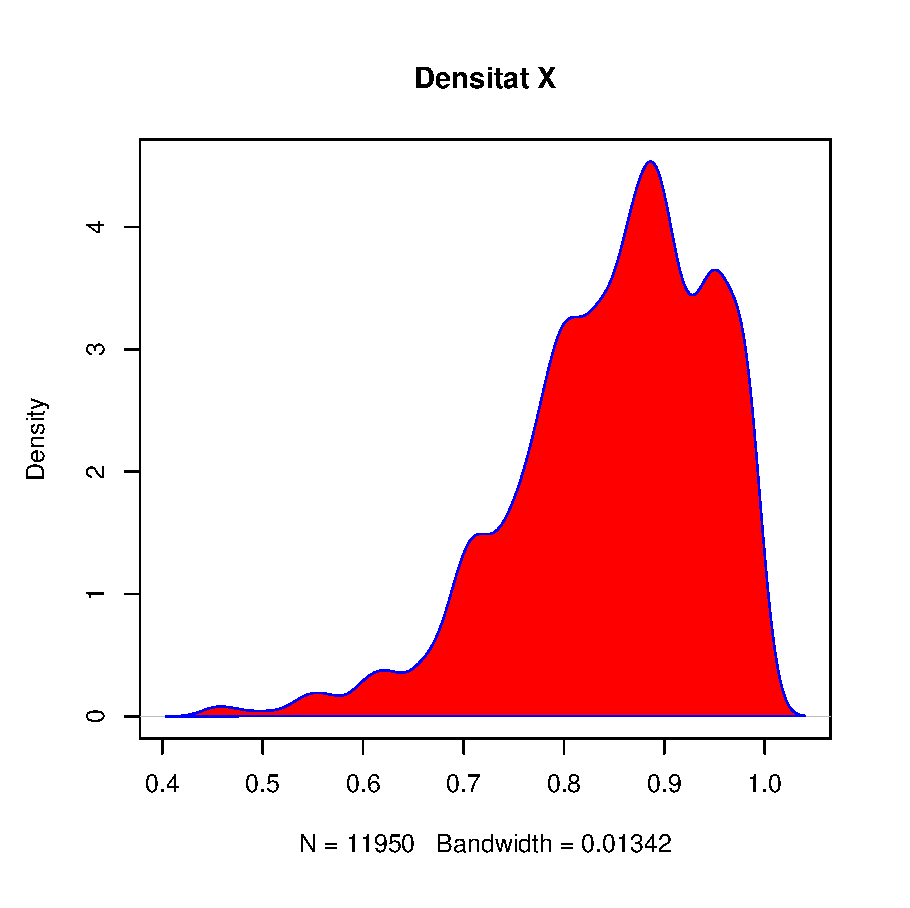
\includegraphics[width=1\linewidth]{./images/no_DENS.eps}
\caption{}
\end{minipage}
\hfill
\begin{minipage}{0.5\linewidth}
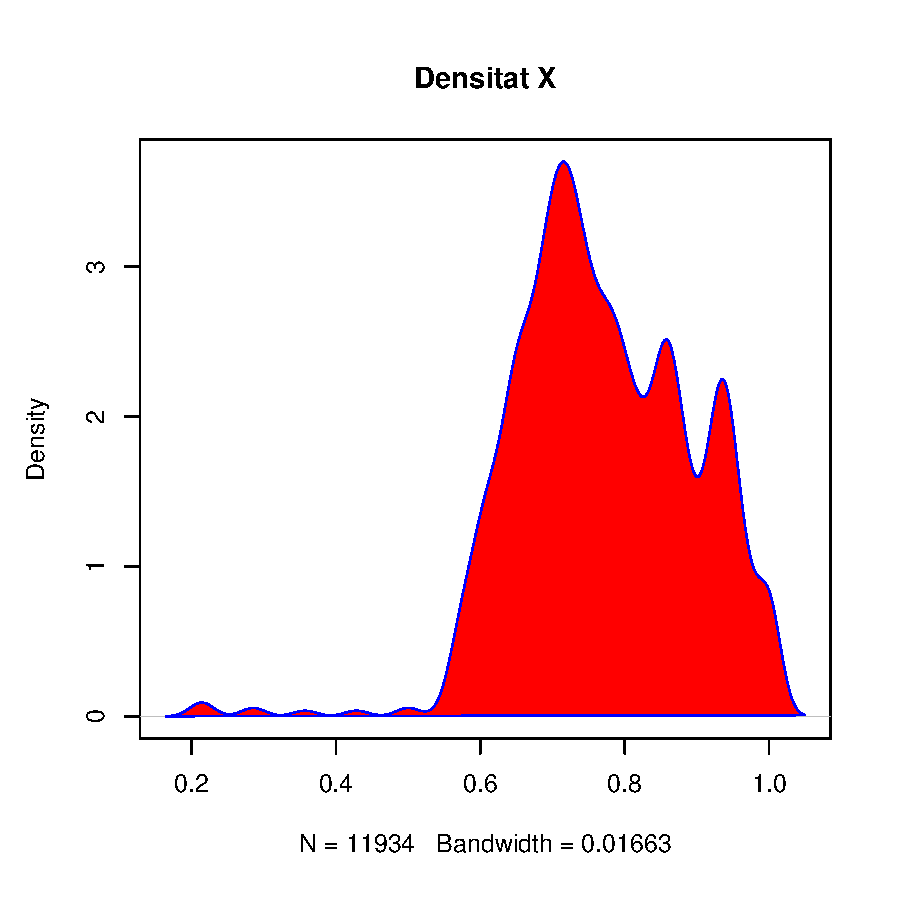
\includegraphics[width=1\linewidth]{./images/si_DENS.eps}
\caption{}
\end{minipage}
\end{figure}
Analitzant les dades obtingudes hem arribat als següents valors:
$$\bar{x} = 0.77083, s^2_x = 0.01459139, n_x = 11934$$
$$\bar{y} = 0.8503347, s^2_y = 0.009507904, n_y = 11950$$
I per tant:
$$\hat{z} = -55.96263$$


El valor de $\hat{z}$ és extremament petit. De fet, calculant el p-valor amb \emph{R} per aquesta $\hat{z}$ el resultat és 0. Per tant, queda clar que s'ha de rebutjar la hipòtesi nul·la. És més, degut a que $\hat{z}$ ha resultat ser negativa, podem afirmar que $\mu_Y > \mu_X$.

\section{Discussió}
\subsection{Prefaci}
El comportament de les variables \emph{X} o \emph{Y} pot dependre de molts factors. Tot seguit n'enumerem uns quants:
\begin{description}
	\item[Hora:] els hàbits rutinaris dels estudiants i els horaris de classe fan que en certes hores hi hagi més gent utilitzant els ordinadors.
	\item[Ocupació de les aules per fer classe:] com més aules estiguin reservades per fer-hi classe, menys ordinadors lliures hi haurà pels estudiants que no tenen classe i en volen fer servir un.
	\item[Exàmens:] els exàmens amb ordinador, a part d'ocupar moltes aules, poden provocar que hi hagi molts estudiants repassant a l'últim moment i que l'ocupació en les hores abans sigui anormalment alta.
\end{description}

\subsection{Conclusió principal}
Hem obtingut que la mitjana d'ocupació a les aules amb classe és inferior a les mitjana de les aules sense classe. Això contradiu la nostra hipòtesis inicial del treball ja que crèiem que les aules amb classe tindrien una ocupació superior a les sense classe. 




\end{document}